\documentclass[../main.tex]{subfiles}

\begin{document}
	\section{Accounting Equations}
	
	\subsection{Return on Assets (ROA)}
	
	Returns on assets is in ratio form as income divided by assets invested \ie 
	
	\[
	\text{ROA} = \frac{\text{Net Profit}}{\text{Average total assets}}
	\]
	
	\subsection{Debt Ratio}
	
	The debt to assets ratio helps evaluate the level of debt risk. We 
	determine a company’s ability to pay it’s debts (liabilities) using the 
	debit ratio. The debt ratio is equal to total liabilities divided by total 
	assets.  
	\[
	\text{Debt Ratio} = \frac{\text{Total Liabilities}}{\text{Total Assets}}
	\]
	A higher ratio indicates that there is greater probability a 
	company will not be able to pay it’s debts in the future.
	
	\subsection{Profit Margin}
	
	Profit margin tells us about the relationship between sales and net 
	profit. We calculate the ratio by dividing net profit for the period by 
	sales revenue.
	
	\[
	\text{Profit Margin} = \frac{\text{Net Profit}}{\text{Net Sales}}
	\]
	
	A high profit margin is an indicator of future growth.
	
	\subsection{Current Ratio}
	
	The current ratio of a company gives us a good indication of the company’s 
	ability to pay its debts when they fall due. The current ratio is 
	calculated by dividing current assets by current liabilities. 
	\[
	\text{Current Ratio} = \frac{\text { Current Assets }}{\text { Current 
	Liabilities }}
	\]
	
	\subsection{Days' Sales Uncollected}
	
	The Days’ Sales Uncollected ratio indicates how much time is likely to pass before we receive cash 
	receipts from credit sales. It is calculated as Accounts Receivable divided by Net Sales times 365 
	days.
	
	\[
	\text{Days' Sales Uncollected} = \frac{\text{Accounts Receivable}}{\text{Net Sales}} \times 365
	\]
	
	
	\subsection{Accounts Receivable Turnover Ratio}
	
	The receivables turnover is the process of selling and collecting on goods 
	and services provided to customers. The process is repeated over and over 
	during each accounting period. The receivables turnover ratio indicates how 
	many times, on average, this process is repeated during the period. 
	
	\[
	\text{Receivable Turnover Ratio} =\frac{\text { Net Sales Revenue }}{\text 
	{ Average Net Receivables}}
	\]
	
	The higher the ratio, the faster the collection of receivables. The faster 
	the collection of receivables, the shorter the company’s operating cycle, 
	which means more cash available for running the business. A low turnover 
	ratio can be a warning sign, suggesting that the company is allowing too 
	much time for customers to pay. When we calculate a ratio and have an 
	income statement item in the numerator and a balance sheet item in the 
	denominator, we must calculate the average balance sheet amount. The 
	quickest way to do this is to add together the beginning and ending balance 
	amounts and divide the total by 2.
	
	If a company offers terms of net 30 on its sales, then one would expect the 
	turnover to be approximately twelve times per year. This ratio should be 
	monitored closely from period to period and should also be used to compare 
	collection trends with that of competitors. 
	
	\begin{figure}[ht]
		\centering
		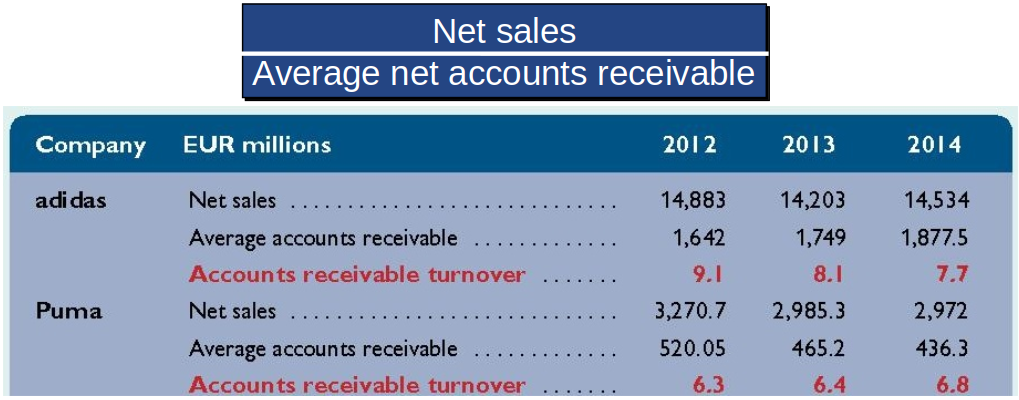
\includegraphics[width=1\columnwidth]{images/c6/turnover_ratio_eg.png}
	\end{figure}
	
	\subsubsection{Days to Collect}
	
	Rather than evaluate the number of times accounts receivable turn over 
	during a year, some people find it easier to think in terms of the length 
	of time (in days) it takes to collect accounts receivable (called days to 
	collect). The Days to Collect measures the average number of days from sale 
	on account to collection of the cash. We divide the Receivable Turnover 
	Ratio into 365, the number of days in most years.
	
	\[
	\text{Days to Collect} = \frac{365}{\text{Receivabel Turnover Ratio}}
	\]
	
	A higher number means a longer time to collect receivables.
	
	
	\subsection{Inventory Turnover}
	
	Inventory turnover is calculated as Cost of Goods Sold divided by Average Inventory. 
	
	\[
	\text{Inventory Turnover}= \frac{\text{Cost of Goods Sold}}{\text{Average Inventory}}
	\]
	This ratio 
	reveals how many times a company turns over (sells) its inventory during a period. If a company’s 
	inventory greatly varies within a year, average inventory amounts can be computed from interim 
	periods such as quarters or months.
	
	Users apply inventory turnover to help analyze short-term liquidity and to assess whether 
	management is doing a good job controlling the amount of inventory available. A low ratio compared 
	to that of competitors suggests inefficient use of assets. The company may be holding more 
	inventory than it needs to support its sales volume. Similarly, a very high ratio compared to that 
	of competitors suggests inventory might be too low. Inventory turnover has no simple rule except 
	to say a high ratio is preferable provided inventory is adequate to meet demand.
	
	\subsection{Days' Sales in Inventory}
	
	Days’ Sales in Inventory is calculated as Ending Inventory divided by Cost of Goods Sold times 365.
	\[
	\text{Days' Sales in Inventory} = \frac{\text{Ending Inventory}}{\text{Cost of Goods Sold}} \times 
	365
	\]
	
	To better interpret inventory turnover, many users measure the adequacy of inventory to meet sales 
	demand. Days’ sales in inventory, also called days’ stock on hand, is a ratio that reveals how 
	much inventory is available in terms of the number of days’ sales. It can be interpreted as the 
	number of days one can sell from inventory if no new items are purchased. This ratio is useful in 
	evaluating liquidity of inventory.
	
	\subsection{Cash Flow on Total Assets}
	
	The Cash Flow on Total Assets ratio is used with profit-based ratios to help assess a company’s performance.  It is calculated as Net cash 
	flow from operating activities divided by Average total assets.
	\[
	\text{Cash Flow on Total Assets} = \frac{\text{Net Cash from Operating Activities}}{\text{Average Total Assets}}
	\]
	This ratio reflects actual cash flows and is not affected by accounting profit recognition and measurement. It can help business decision 
	makers estimate the amount and timing of cash flows when planning and analyzing operating activities.
	
\end{document}